% !TEX TS-program = xelatex
% !TEX encoding = UTF-8 Unicode

\documentclass[AutoFakeBold]{LZUThesis}
\usepackage{wasysym}
\usepackage{enumitem}
\usepackage[most]{tcolorbox}
\usepackage{multirow}
\usepackage{tikz}
\usetikzlibrary{arrows.meta, decorations.markings}
\usepackage{hyperref}
\usepackage[numbers,sort&compress]{natbib}
\newcommand{\upcite}[1]{\textsuperscript{\textsuperscript{\cite{#1}}}}
\allowdisplaybreaks[4]

% for verilog code coloring
\definecolor{vgreen}{RGB}{104,180,104}
\definecolor{vblue}{RGB}{49,49,255}
\definecolor{vorange}{RGB}{255,143,102}

\lstdefinestyle{verilog-style}
{
    language=Verilog,
    basicstyle=\small\ttfamily,
    keywordstyle=\color{vblue},
    identifierstyle=\color{black},
    commentstyle=\color{vgreen},
    numbers=left,
    numberstyle=\tiny\color{black},
    numbersep=10pt,
    tabsize=8,
    moredelim=*[s][\colorIndex]{[}{]},
    literate=*{:}{:}1
}

\makeatletter
\newcommand*\@lbracket{[}
\newcommand*\@rbracket{]}
\newcommand*\@colon{:}
\newcommand*\colorIndex{%
    \edef\@temp{\the\lst@token}%
    \ifx\@temp\@lbracket \color{black}%
    \else\ifx\@temp\@rbracket \color{black}%
    \else\ifx\@temp\@colon \color{black}%
    \else \color{vorange}%
    \fi\fi\fi
}
\makeatother

\usepackage{trace}

\begin{document}

\title{{实验五 存储器实现}}

\entitle{Experiment 5 Memory Implementation}

\author{生物信息学班 李泽华 320210928501}
\major{计算机组成原理}
\advisor{高平}
\college{生命科学学院}
\grade{2021级}


\frontmatter

% \ZhAbstract{
% }{
% }

%\EnAbstract{
%}{
%}

%\customcontent

\mainmatter

% \chapter{\texorpdfstring{绪 \quad 论}{绪论}}
\chapter{实验目的}
\begin{itemize}
    \item 了解只读存储器 ROM 和随机存取存储器 RAM 的原理。
    \item 理解 ROM 读取数据及 RAM 读取、写入数据的过程。
    \item 理解计算机中存储器地址编址和数据索引方法。
    \item 理解同步 RAM 和异步 RAM 的区别。
    \item 掌握调用 Xilinx 库 IP 实例化 RAM 的设计方法。
    \item 熟悉并运用 verilog 语言进行电路设计。
    \item 为后续设计 cpu 的实验打下基础。
\end{itemize}
\chapter{实验任务与要求}
\section{试验任务}
\begin{itemize}
    \item 学习存储器的设计及原理,如:ROM 读地址索引读取数据过程及时序,RAM 读写时序,同步和异步的区别等。
    \item 学习计算机中内存地址编址和数据索引方法。
    \item 自行设计本次实验的方案,画出结构框图,详细标出输入输出端口,确定存储器宽度、深度和写使能位数。
    \item 学习 Vivado 工具中调用库 IP 的方法。
    \item 本次实验要求调用 Xilinx 库 IP 实例化一块 RAM。实例化的 RAM 选择为同步RAM。本次实验的 RAM 建议设置为两个端口,一个端口用来正常的读写,另一个端口作为调试端口只使用读功能用于观察存储器内部数据。
    \item 调用 Xilinx 库 IP 实例化一块 RAM,并进行仿真,得到正确的波形图。
    \item 将以上设计作为一个单独的模块,设计一个外围模块去调用该模块。外围模块中需调用封装好的 LCD 触摸屏模块,显示 RAM 的正常端口的地址、待写入的数据和读出的数据,显示调试端口的地址和读出的数据。并且需要利用触摸功能输入正常端口的地址和写数据,以及调试端口的地址
    \item 将编写的代码进行综合布局布线,并下载到实验箱中的 FPGA 板子上进行演示。
\end{itemize}

注意:存储器深度不要过大,避免耗费过多的 FPGA 上的资源。本次实验要求实现
同步的存储器。而异步存储器的搭建方法同寄存器堆的搭建,但不同的是,寄存器堆
中读写端口是分开的,但对于异步 RAM 要求读写共用一个端口,只是会增加一个写使
能信号。可以自行尝试搭建异步的 ROM 和 RAM,在单周期 CPU 实验中会用到异步的 ROM
作为指令存储器,而异步 RAM 作为数据存储器。
\section{实验要求}
\begin{enumerate}
    \item 实验箱结果截图
    \item 核心代码注释
    \item 解释同步方式和异步方式访问存储时的差异(控制信号以及访问流程)
\end{enumerate}

\chapter{实验结果}
\section{实验代码与注释}
\subsection{data ram}
\lstinputlisting[style=verilog-style]{F:/Onedrive/study/programing/ComputerCompositionPrinciples/exp/lihuax/5_memory/exp/src/memory_async/data_ram/data_ram.v}
\subsection{inst rom}
\lstinputlisting[style=verilog-style]{F:/Onedrive/study/programing/ComputerCompositionPrinciples/exp/lihuax/5_memory/exp/src/memory_async/inst_rom/inst_rom.v}

\section{上机结果}
\begin{figure}[htbp]
    \centering
    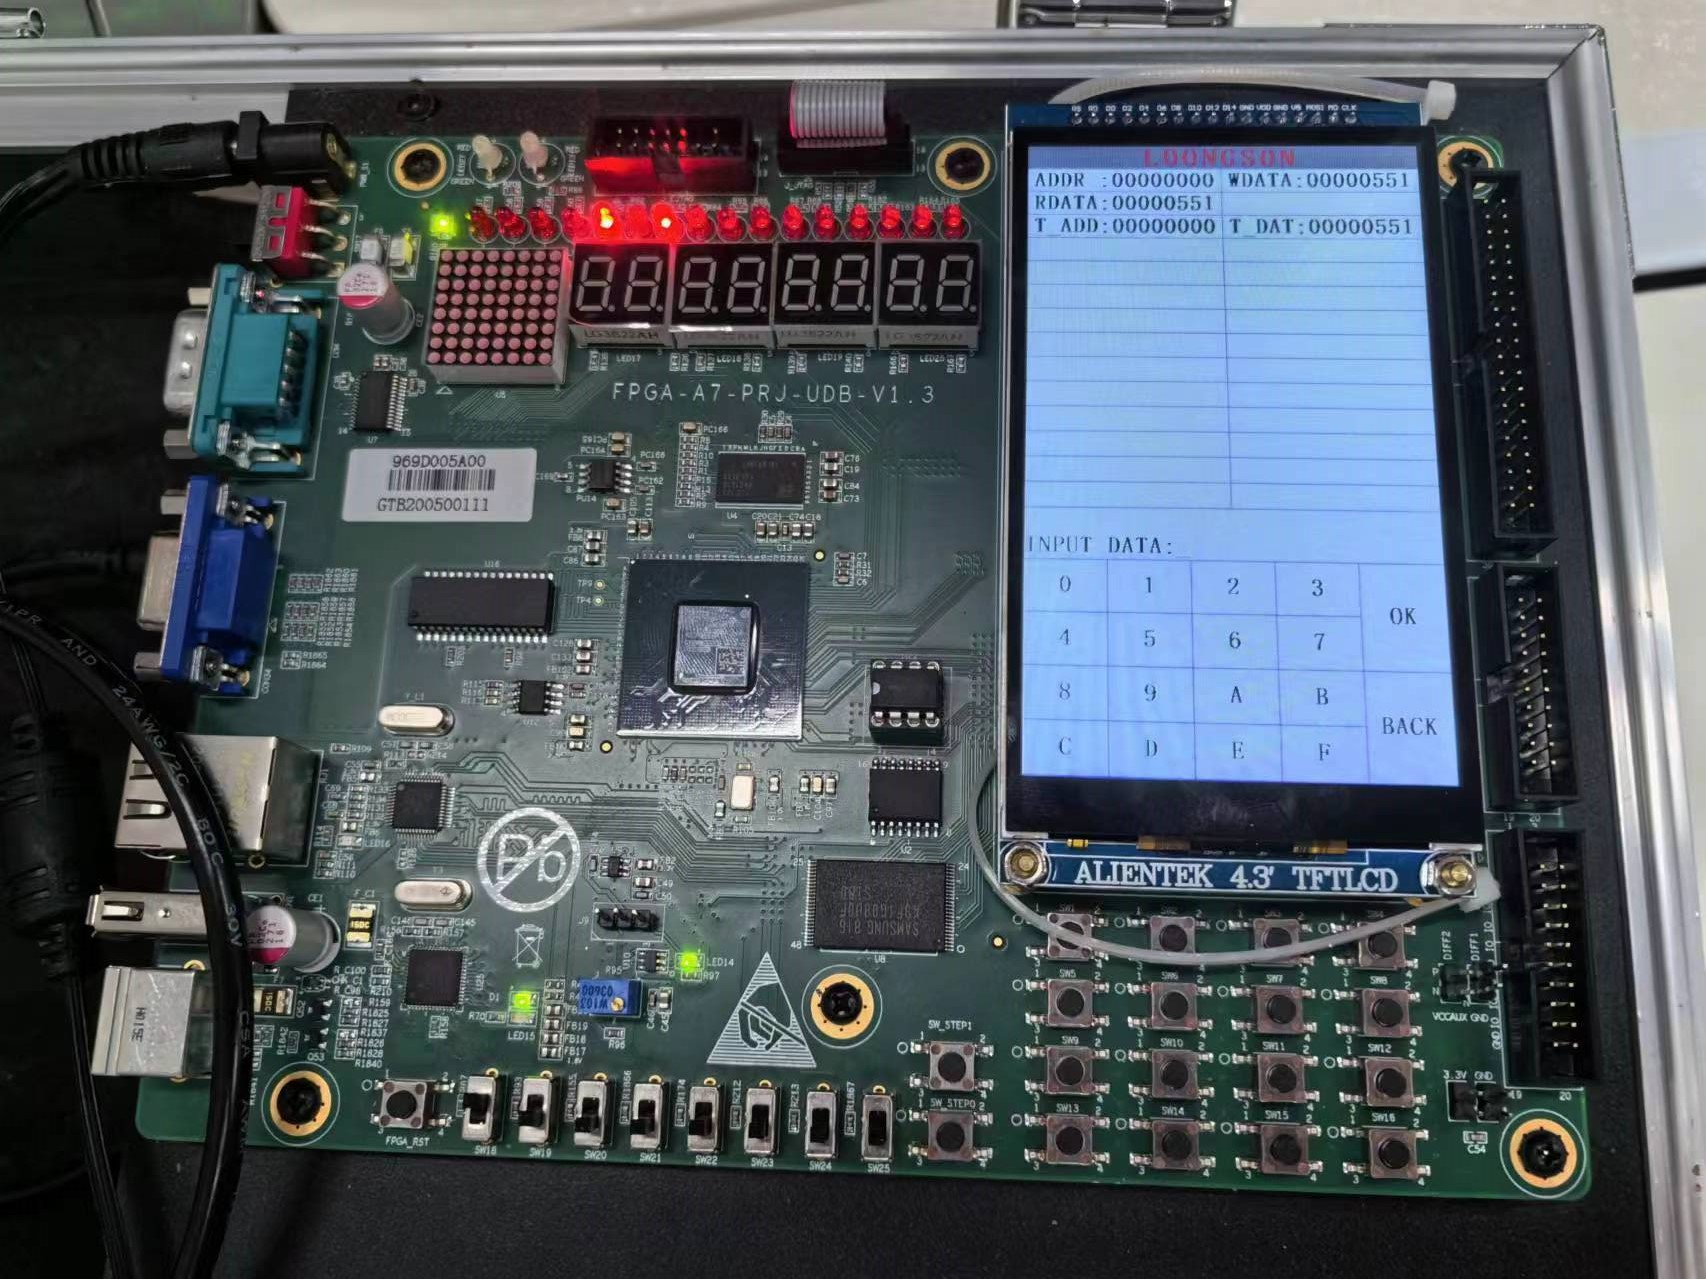
\includegraphics[width=0.7\textwidth]{img/fpga}
    \caption{上机结果}
\end{figure}

\chapter{思考与讨论}
\subsection*{同步访问}

同步访问是指数据传输或访问过程与系统时钟同步进行。在同步系统中,所有操作(如读取和写入)都在时钟信号的特定边缘触发,例如在时钟的上升沿或下降沿。

\textbf{控制信号:}
\begin{itemize}
    \item \textbf{时钟信号(Clock)}:这是同步访问的核心,所有操作都根据这个时钟信号的节拍进行。
    \item \textbf{使能信号(Enable)}:决定何时可以对存储设备进行访问。
    \item \textbf{读/写信号(Read/Write)}:指示进行的是读操作还是写操作。
\end{itemize}

\textbf{访问流程:}
\begin{enumerate}
    \item 系统时钟产生节拍:确定操作的具体时机。
    \item 设置地址和数据:在时钟信号到来之前,地址和数据线被设置。
    \item 使能信号激活:允许数据在指定的时钟边缘被读取或写入。
    \item 读/写操作执行:根据时钟信号的触发,执行读或写操作。
    \item 数据稳定:数据在下一个时钟信号到来前保持稳定,以确保数据正确读取或写入。
\end{enumerate}

\subsection*{异步访问}

异步访问不依赖于系统的主时钟信号,而是使用控制信号来直接管理读写操作的时序。

\textbf{控制信号:}
\begin{itemize}
    \item \textbf{请求信号(Request)}:用来从主设备向存储设备发起访问请求。
    \item \textbf{就绪/应答信号(Ready/Acknowledge)}:存储设备用它来响应主设备的请求,表示数据已经准备好或已成功接收。
    \item \textbf{读/写信号}:与同步方式相同,指示进行的是读操作还是写操作。
\end{itemize}

\textbf{访问流程:}
\begin{enumerate}
    \item 请求信号发起:主设备发出请求信号,要求进行数据读取或写入。
    \item 设置地址和数据:如果是写操作,数据会与请求一同发送。
    \item 等待就绪/应答信号:存储设备在数据准备就绪或接收完毕后,发回应答信号。
    \item 执行读/写操作:在接收到应答信号后,完成数据传输。
    \item 完成操作:操作完成后,请求和应答信号被撤销,系统进入下一状态。
\end{enumerate}

\textbf{总结}

同步访问与系统时钟紧密相关,需要所有操作严格按照时钟信号进行,适合于速度要求严格且时序要求高的环境。异步访问则更灵活,不依赖时钟信号,适合于时钟不方便传递或者设备之间时钟不同步的情况。两者的选择取决于具体的系统设计和


%\section{课后问题}
%论文后部
\backmatter


%=======%
%引入参考文献文件
%=======%
%\bibdatabase{bib/database}%bib文件名称 仅修改bib/ 后部分
%\printbib
%\nocite{*} %显示数据库中有的,但是正文没有引用的文献



\Appendix
参考链接:
\url{https://github.com/zehua0417/ComputerOrganizationAndArchitecture_exp}
\begin{figure}[htbp]
    \centering
    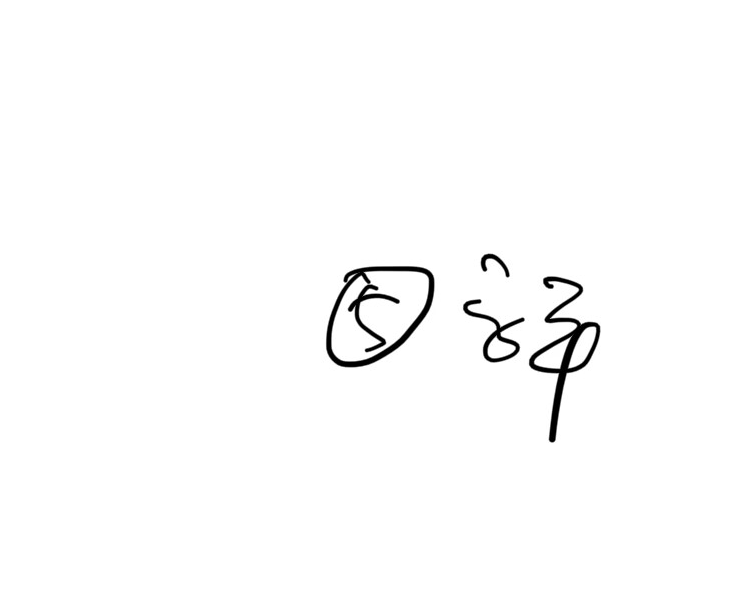
\includegraphics[width=0.4\textwidth]{img/sign}
\end{figure}

%\Thanks


%\Grade %这一句才是成绩页,上面是填写


\end{document}
